\documentclass[conference]{IEEEtran}

\usepackage[spanish,es-nodecimaldot]{babel}
\usepackage[utf8]{inputenc}
\usepackage[T1]{fontenc}
\usepackage{graphicx}
\usepackage{listings}
\usepackage{xcolor}
\usepackage{url}
\usepackage{booktabs}
\usepackage{amsmath}

\lstset{
  basicstyle=\ttfamily\scriptsize,
  keywordstyle=\color{blue!60!black},
  commentstyle=\color{gray},
  stringstyle=\color{green!40!black},
  breaklines=true,
  frame=single,
  captionpos=b,
  upquote=true,
  showstringspaces=false,
  columns=flexible,
  keepspaces=true
}

\begin{document}

\title{Descomposición de un conjunto de datos plano en un modelo
relacional normalizado y su explotación mediante consultas SQL}

\author{\IEEEauthorblockN{Juan Esteban Tibamoso Sánchez - 30000131944}
\IEEEauthorblockA{Facultad de Ingeniería - Ingeniería Multimedia\\
Universidad de San Buenaventura\\
Bogotá, Colombia}}

\maketitle

\begin{abstract}
Se transformó un archivo plano de 4.070 partidos de la Premier League,
correspondiente a once temporadas, en un modelo relacional normalizado hasta
tercera forma normal. El dataset presentaba un grupo repetitivo que duplicaba
catorce atributos por bando dentro de la misma fila, y tres columnas cuyo
contenido era derivable de otras. La descomposición produjo cuatro relaciones
articuladas por una tabla puente que resuelve la cardinalidad entre partidos y
equipos. El esquema se implementó en MySQL y se pobló mediante un programa de
carga en Node.js que valida cada registro antes de insertarlo. Sobre el modelo
resultante se formularon ocho consultas de análisis cuyos hallazgos principales
contradicen expectativas intuitivas: el liderato histórico no se explica por el
volumen de partidos disputados, casi la mitad de las victorias se obtuvieron
con posesión minoritaria, y la temporada más sancionada con tarjetas rojas fue
también la de menor producción ofensiva.
\end{abstract}

\begin{IEEEkeywords}
Modelo relacional, normalización, tercera forma normal, SQL, MySQL, ETL,
análisis de datos.
\end{IEEEkeywords}

%=======================================================================
\section{Introducción}

En la ciencia de datos y la ingeniería de software, existe una distinción
fundamental entre el almacenamiento plano de información y el modelado
relacional estructurado. Mientras que un archivo plano (como un CSV) actúa como
un contenedor estático diseñado para el transporte de datos, una base de datos
relacional modela las reglas, restricciones y entidades del dominio. La
principal limitación de una tabla plana emerge al realizar análisis complejos:
obliga a realizar lecturas extensivas y redundantes de columnas, dificultando
la formulación de consultas eficientes que respondan a la lógica real del
negocio o dominio estudiado.

El presente trabajo aborda esta problemática mediante la transformación de un
conjunto de datos crudo correspondiente a 4.070 partidos de la Premier League a
lo largo de once temporadas. En su estado inicial, el dataset presentaba una
estructura desnormalizada de 33 columnas que duplicaba catorce atributos
estadísticos por bando (local y visitante) dentro de una misma fila, además de
incluir variables cuyos valores eran derivables de forma analítica. Esta
organización, aunque funcional para el intercambio masivo de datos, enmascara
la naturaleza del dominio deportivo, donde un encuentro no posee estadísticas
directas, sino que consolida el desempeño independiente de dos equipos
interactuando en un mismo evento.

Para resolver estas inconsistencias, se llevó a cabo un proceso de
descomposición guiado por la teoría de la normalización. No se buscó trasladar
ciegamente la estructura del archivo a una base de datos, sino descomponerla
mediante dependencias funcionales secuenciales hasta alcanzar la Tercera Forma
Normal (3FN). Como resultado, se diseñó e implementó un modelo de cuatro
relaciones interconectadas por una tabla puente en MySQL, alimentado mediante
un script de validación y carga en Node.js.

Finalmente, la validez y utilidad del modelo relacional construido se demuestra
mediante la formulación y ejecución de ocho consultas SQL analíticas. Los
hallazgos obtenidos ponen de manifiesto la importancia de estructurar
correctamente los datos: revelan patrones contraintuitivos sobre la posesión de
balón, la eficiencia ofensiva y la disciplina deportiva que no habrían sido
evidentes mediante el análisis de la tabla plana original.

El código fuente completo del esquema, el programa de carga y las ocho
consultas se encuentra disponible en
\url{https://github.com/tibamosojuan-jpg/lab-sql-futbol}.

%=======================================================================
\section{Objetivos}

\subsection{Objetivo general}

Transformar un conjunto de datos crudo y no normalizado en un modelo relacional
consistente, justificando técnicamente cada decisión de exclusión de
información y cada paso de normalización, y explotar ese modelo mediante
consultas SQL que respondan preguntas concretas de análisis.

\subsection{Objetivos específicos}

\begin{enumerate}
\item Identificar las dependencias funcionales presentes en la tabla plana y
descomponerla aplicando primera, segunda y tercera forma normal como pasos
secuenciales justificados.

\item Implementar el esquema normalizado en MySQL y desarrollar un programa de
carga en Node.js que valide los registros de entrada y reporte explícitamente
los rechazos de inserción.

\item Formular consultas SQL orientadas a preguntas de análisis e interpretar
sus resultados en términos del dominio, distinguiendo lo que el dato muestra de
lo que la intuición anticiparía.
\end{enumerate}

%=======================================================================
\section{Marco teórico}

\subsection{Dependencia funcional}

Un atributo $B$ depende funcionalmente de un atributo $A$, denotado $A
\rightarrow B$, si cada valor de $A$ determina un único valor de $B$. Las
dependencias funcionales son el instrumento con el que se decide cómo
descomponer una relación: no dependen de los datos que la tabla contiene en un
momento dado, sino de las reglas del dominio que modela \cite{elmasri}.

\subsection{Formas normales}

La normalización es un proceso de descomposición sucesiva que elimina
redundancia y previene anomalías de inserción, actualización y borrado
\cite{date}.

La \textbf{primera forma normal} exige que cada atributo sea atómico y que no
existan grupos repetitivos, es decir, conjuntos de columnas que representen el
mismo atributo medido sobre sujetos distintos.

La \textbf{segunda forma normal} exige, sobre una relación en 1FN con clave
primaria compuesta, que todo atributo no clave dependa de la clave completa y
no de una parte de ella. Una dependencia parcial indica que ese atributo
pertenece a una entidad distinta.

La \textbf{tercera forma normal} exige que ningún atributo no clave dependa de
otro atributo no clave. Esas dependencias transitivas son la forma en que una
entidad ajena queda escondida dentro de la tabla \cite{elmasri}.

\subsection{Relaciones N:M y tablas puente}

El modelo relacional no admite representar directamente una cardinalidad de
muchos a muchos entre dos entidades. La resolución canónica consiste en
introducir una tercera relación cuya clave primaria es la combinación de las
claves foráneas de ambas entidades. Esa relación intermedia no es un artificio
técnico: suele corresponder a una entidad real del dominio que la lectura
inicial pasó por alto \cite{connolly}.

\subsection{Datos derivados}

Un atributo calculable a partir de otros atributos de la misma relación
introduce una dependencia transitiva y, con ella, riesgo de inconsistencia: si
el valor base cambia y el derivado no se recalcula, la base de datos sostiene
simultáneamente dos versiones de un mismo hecho. La recomendación general es
calcularlos en consulta en lugar de almacenarlos \cite{date}.

%=======================================================================
\section{Análisis del dataset y selección de información}

El archivo contiene 4.070 registros correspondientes a once temporadas, desde
la 10/11 hasta la 20/21, y 37 equipos distintos. No presenta valores nulos en
ninguna columna. La tripleta formada por fecha, equipo local y equipo visitante
identifica unívocamente cada fila, sin repeticiones.

Dos temporadas son parciales. La 20/21 contiene 271 partidos con corte el 7 de
marzo de 2021, y la 15/16 registra 379 en lugar de 380. Esta observación no
afecta el modelo, pero condiciona la interpretación de cualquier agregado por
temporada, como se discute en la Sección~\ref{sec:analisis}.

Tres columnas se excluyeron de la carga. La exclusión no obedece a criterios de
limpieza sino a que almacenarlas violaría la tercera forma normal.

La columna \texttt{X} es el índice de fila del archivo. No corresponde a ningún
atributo del dominio y su valor depende del orden en que el archivo fue
generado, no del partido que describe.

La columna \texttt{sg\_match\_ft} equivale exactamente a la diferencia entre
\texttt{goal\_home\_ft} y \texttt{goal\_away\_ft}. Se verificó la igualdad en
las 4.070 filas sin excepciones.

La columna \texttt{result} codifica el desenlace del encuentro mediante los
valores 0 para victoria local, 1 para victoria visitante y 2 para empate. Se
verificó que la codificación es consistente en todo el archivo. Al igual que la
anterior, su contenido se deduce íntegramente de los goles de ambos bandos.

Las dos últimas comparten el mismo defecto: son hechos derivados almacenados
como si fueran hechos primarios. Si un gol se corrigiera sin actualizar el
derivado, la base quedaría afirmando dos cosas incompatibles sobre el mismo
partido. Ambas se calculan en consulta cuando se necesitan, como se observa en
la expresión \texttt{CASE} que construye la tabla de posiciones en la
Sección~\ref{sec:analisis}.

Las veintiocho columnas de estadísticas restantes se conservaron. El criterio
es el enunciado al inicio: el sistema modela rendimiento deportivo, y esas
métricas constituyen precisamente el objeto de análisis, no información
accesoria.

%=======================================================================
\section{Modelo de datos y normalización}

\subsection{Punto de partida}

El archivo constituye una única relación universal en la que cada fila contiene
el partido completo. La descomposición que sigue presenta cada forma normal
como un paso independiente con su justificación.

\subsection{Primera forma normal}

El dataset presenta un grupo repetitivo que no es evidente a primera vista
porque está expresado mediante nombres de columna distintos.
\texttt{home\_shots} y \texttt{away\_shots} no son dos atributos diferentes:
son el mismo atributo medido sobre dos sujetos distintos. El patrón se repite
en posesión, pases, toques, entradas, despejes, córners, fueras de juego,
faltas, tarjetas amarillas, tarjetas rojas, tiros a puerta y goles. Catorce
atributos duplicados por bando.

La corrección no consiste en renombrar columnas sino en cambiar la unidad que
representa la fila. En lugar de un registro por partido con dos bandos adentro,
se pasa a un registro por cada participación de un equipo en un partido. De ahí
surge la relación \texttt{game\_team\_stat}, con una columna \texttt{role} que
distingue la condición de local o visitante.

Esta es la relación puente que resuelve la cardinalidad de muchos a muchos
entre partidos y equipos: un partido involucra dos equipos y un equipo
participa en muchos partidos. El efecto es medible: las 4.070 filas del archivo
se convierten en 8.140 registros de participación.

\subsection{Segunda forma normal}

La relación obtenida tiene clave primaria compuesta por el identificador del
partido y el del equipo. Bajo esa clave, la fecha y la temporada presentan una
dependencia parcial: ambas quedan determinadas únicamente por el partido, sin
importar qué equipo de los dos se considere. Un partido se jugó un solo día,
cualquiera sea el bando desde el que se lo mire.

Esa dependencia parcial señala una entidad distinta oculta en la relación. Se
extrae \texttt{game}, que concentra los atributos propios del encuentro, y
\texttt{game\_team\_stat} conserva únicamente aquellos que dependen de la
combinación completa de partido y equipo, es decir, el desempeño individual.

\subsection{Tercera forma normal}

Persisten dos dependencias transitivas.

La primera involucra la temporada. Esta no depende directamente del partido
sino de su fecha, formando la cadena \texttt{game\_id} $\rightarrow$
\texttt{played\_on} $\rightarrow$ \texttt{season}. Se verificó que los rangos
de fechas de las once temporadas no se solapan, lo que confirma que la fecha
determina unívocamente la temporada. Se extrae la relación \texttt{season}.

La segunda involucra el nombre del equipo, determinado por su identificador y
no por la participación particular. Mantenerlo en la tabla puente repetiría la
cadena de texto en cada uno de los 8.140 registros, con la consiguiente
anomalía de actualización si un club cambiara de denominación. Se extrae la
relación \texttt{team}.

A este paso corresponden también las exclusiones de \texttt{sg\_match\_ft} y
\texttt{result} discutidas en la sección anterior, por ser atributos
determinados por otros atributos no clave.

\subsection{Esquema resultante}

La Fig.~\ref{fig:modelo} presenta el modelo final. Las cuatro relaciones se
articulan en tres vínculos: una temporada agrupa muchos partidos, un partido
genera exactamente dos participaciones y un equipo acumula muchas
participaciones a lo largo del tiempo.

\begin{figure}[htbp]
\centering
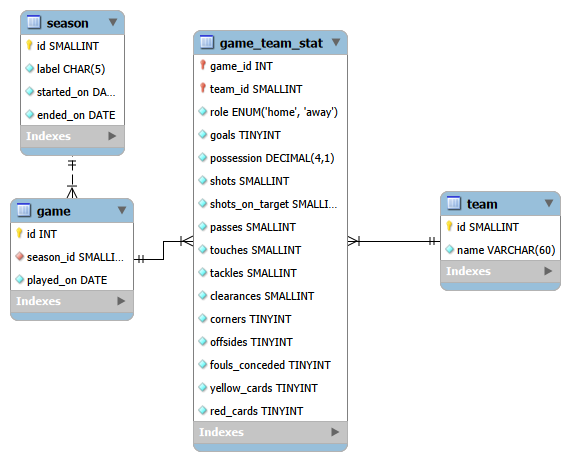
\includegraphics[width=\columnwidth]{diagrama.png}
\caption{Modelo entidad-relación normalizado en tercera forma normal.
\texttt{game\_team\_stat} opera como tabla puente entre \texttt{game} y
\texttt{team}.}
\label{fig:modelo}
\end{figure}

\subsection{Una concesión del diseño}

Llevar la descomposición hasta este punto tiene un costo que conviene declarar.
Al trasladar la condición de local y visitante por completo a la tabla puente,
la relación \texttt{game} queda sin clave natural: solo almacena temporada y
fecha, y varios partidos comparten ambos valores. El esquema no puede, por sí
solo, impedir que el mismo encuentro se inserte dos veces.

La restricción \texttt{UNIQUE (game\_id, role)} mitiga parcialmente el problema
al garantizar que ningún partido registre dos locales o dos visitantes, y el
programa de carga procesa el archivo una sola vez. La alternativa habría sido
conservar referencias al equipo local y al visitante dentro de \texttt{game},
lo que restituiría una clave natural a costa de reintroducir el grupo
repetitivo que la 1FN eliminó. Se privilegió la integridad del modelo sobre la
comodidad de la restricción.

%=======================================================================
\section{Implementación del esquema y programa de carga}

\subsection{Traducción a DDL}

El esquema se implementó en MySQL sobre el motor InnoDB \cite{mysql}. Los tipos se
dimensionaron según los rangos observados en el dataset: \texttt{TINYINT
UNSIGNED} para goles y tarjetas, \texttt{SMALLINT UNSIGNED} para tiros, pases y
toques, y \texttt{DECIMAL(4,1)} para la posesión, que el archivo expresa con un
decimal.

Se declararon dos restricciones de verificación. La primera limita la posesión
al rango entre 0 y 100. La segunda exige que los tiros a puerta no superen el
total de tiros.

\begin{lstlisting}[language=SQL,caption={Restricciones de la tabla puente}]
PRIMARY KEY (game_id, team_id),
UNIQUE KEY uq_game_role (game_id, role),
CONSTRAINT chk_possession_range
    CHECK (possession BETWEEN 0 AND 100),
CONSTRAINT chk_shots_on_target
    CHECK (shots_on_target <= shots)
\end{lstlisting}

Una tercera restricción aparentemente razonable fue descartada tras verificarla
contra el dataset. Exigir que los goles no superen los tiros a puerta
rechazaría 16 registros legítimos, en los que un equipo anotó mediante autogol
del rival: el gol se contabiliza para el equipo pero el disparo no se le
atribuye. El caso ilustra que una restricción de integridad debe derivarse de
las reglas del dominio y no de la intuición sobre los datos.

\subsection{Decisión arquitectónica del programa de carga}

El programa se implementó como script independiente y no siguiendo la
arquitectura por capas de un servicio web. La justificación es que la carga es
un proceso de ejecución única, sin superficie HTTP ni consumo desde un cliente
externo: montar rutas y controladores sobre él añadiría indirección sin
estructura, puesto que no existe petición que enrutar ni respuesta que
serializar.

Esa decisión no implicó renunciar a la separación de responsabilidades, que se
resolvió por módulo. La lectura del origen, la traducción al modelo, la
persistencia y la orquestación residen en archivos distintos, de modo que un
cambio en el formato del archivo de entrada no toca el código que inserta en la
base de datos.

\subsection{Validación y manejo de errores}

Cada fila atraviesa una etapa de validación antes de tocar la base de datos. Se
verifica la presencia y el tipo de los campos obligatorios, el formato ISO de
la fecha y la coherencia básica del registro, incluyendo que un equipo no
figure como rival de sí mismo.

Las fallas se tratan por registro y no por lote. Si una fila es rechazada, el
error se captura junto con su número de línea y el código devuelto por MySQL, y
el proceso continúa con las restantes. Al final se reporta el conteo de
rechazos y el detalle de los primeros casos.

El comportamiento se comprobó de forma no intencionada al ejecutar la carga
sobre una base ya poblada. El programa reportó 4.060 rechazos con código
\texttt{ER\_DUP\_ENTRY} sobre la clave única de temporada, y la verificación
posterior confirmó que los datos existentes permanecieron intactos. La carga
falló, pero no en silencio, que es exactamente el comportamiento buscado.

\subsection{Verificación de la carga}

\begin{table}[htbp]
\caption{Registros cargados por relación}
\label{tab:carga}
\centering
\begin{tabular}{lr}
\toprule
\textbf{Relación} & \textbf{Registros} \\
\midrule
\texttt{season}           & 11 \\
\texttt{team}             & 37 \\
\texttt{game}             & 4.070 \\
\texttt{game\_team\_stat} & 8.140 \\
\bottomrule
\end{tabular}
\end{table}

La Tabla~\ref{tab:carga} recoge el resultado. Los 4.070 partidos corresponden
uno a uno con las filas del archivo y las 8.140 participaciones confirman la
duplicación esperada por la descomposición de 1FN.

Se añadieron dos comprobaciones de integridad que el conteo por sí solo no
detecta. La primera verifica que todo partido tenga exactamente dos
participantes; la segunda, que la posesión de cada encuentro sume 100. Ambas
devolvieron cero incidencias.

%=======================================================================
\section{Consultas básicas}

Ninguna consulta de esta sección emplea \texttt{SELECT *}. Cada una proyecta
únicamente las columnas necesarias para responder la pregunta que la motiva.

\subsection{Filtrado compuesto}

\emph{¿En qué participaciones un equipo anotó cuatro o más goles teniendo menos
del 45\% de la posesión?}

\begin{lstlisting}[language=SQL]
SELECT t.name AS team, g.played_on, s.goals,
       s.possession, s.shots_on_target
FROM game_team_stat AS s
JOIN team AS t ON t.id = s.team_id
JOIN game AS g ON g.id = s.game_id
WHERE s.goals >= 4
  AND s.possession < 45
ORDER BY s.goals DESC, s.possession ASC
LIMIT 15;
\end{lstlisting}

\begin{table}[htbp]
\caption{Goleadas con posesión inferior al 45\% (extracto)}
\label{tab:filtrado}
\centering
\begin{tabular}{llrrr}
\toprule
\textbf{Equipo} & \textbf{Fecha} & \textbf{G} & \textbf{Pos.} & \textbf{TaP} \\
\midrule
Aston Villa       & 2020-10-04 & 7 & 30,2 & 11 \\
Arsenal           & 2012-12-29 & 7 & 44,2 & 10 \\
Southampton       & 2015-05-16 & 6 & 35,6 & 11 \\
Chelsea           & 2014-08-30 & 6 & 38,5 & 8  \\
Manchester United & 2020-12-20 & 6 & 41,5 & 14 \\
Newcastle United  & 2015-10-18 & 6 & 44,2 & 6  \\
\bottomrule
\end{tabular}
\end{table}

Como recoge la Tabla~\ref{tab:filtrado}, la condición se satisface en 69
participaciones. El caso extremo es Aston Villa el 4 de octubre de 2020, con
siete goles y 30,2\% de posesión. Los \texttt{JOIN} cumplen aquí una función de
legibilidad: sin ellos el resultado devolvería identificadores numéricos sin
referente. Lo que la consulta demuestra es el filtrado por condiciones
combinadas.

\subsection{Reunión entre dos entidades}

\emph{¿Qué equipos registran las diez posesiones más altas del histórico?}

\begin{lstlisting}[language=SQL]
SELECT t.name AS team, s.possession, s.passes, s.goals
FROM game_team_stat AS s
JOIN team AS t ON t.id = s.team_id
ORDER BY s.possession DESC
LIMIT 10;
\end{lstlisting}

\begin{table}[htbp]
\caption{Posesiones más altas del histórico (extracto)}
\label{tab:posesion}
\centering
\begin{tabular}{lrrr}
\toprule
\textbf{Equipo} & \textbf{Posesión} & \textbf{Pases} & \textbf{Goles} \\
\midrule
Manchester City   & 82,9 & 1.015 & 5 \\
Manchester City   & 82,0 & 976   & 3 \\
Manchester City   & 82,0 & 809   & 1 \\
Manchester City   & 81,3 & 710   & 3 \\
Huddersfield Town & 81,2 & 679   & 0 \\
Chelsea           & 81,1 & 913   & 2 \\
\bottomrule
\end{tabular}
\end{table}

En la Tabla~\ref{tab:posesion} se observa que Manchester City ocupa cinco de
las diez posiciones, encabezadas por un 82,9\% con 1.015 pases. El dato que
anticipa la Sección~\ref{sec:analisis} está en la quinta fila: Huddersfield
Town registró 81,2\% de posesión y cero goles.

\subsection{Reunión entre cuatro entidades}

\emph{¿Cuántos goles anotó cada equipo en la temporada 20/21?}

\begin{lstlisting}[language=SQL]
SELECT t.name AS team, se.label AS season,
       SUM(s.goals) AS goals
FROM game_team_stat AS s
JOIN team   AS t  ON t.id = s.team_id
JOIN game   AS g  ON g.id = s.game_id
JOIN season AS se ON se.id = g.season_id
WHERE se.label = '20/21'
GROUP BY t.id, t.name, se.label
ORDER BY goals DESC;
\end{lstlisting}

\begin{table}[htbp]
\caption{Goles por equipo en la temporada 20/21 (extracto)}
\label{tab:goles2021}
\centering
\begin{tabular}{llr}
\toprule
\textbf{Equipo} & \textbf{Temporada} & \textbf{Goles} \\
\midrule
Manchester City   & 20/21 & 56 \\
Manchester United & 20/21 & 55 \\
Leicester City    & 20/21 & 48 \\
Liverpool         & 20/21 & 47 \\
Leeds United      & 20/21 & 43 \\
Chelsea           & 20/21 & 42 \\
\bottomrule
\end{tabular}
\end{table}

La consulta recorre las cuatro relaciones del modelo y evidencia que la
descomposición no obstaculiza la reconstrucción de la vista original. Según la
Tabla~\ref{tab:goles2021}, Manchester City encabeza con 56 goles, seguido por
Manchester United con 55.

\subsection{Agregación con agrupamiento}

\emph{¿Cómo evoluciona la disciplina por temporada, medida en tarjetas
amarillas por partido?}

\begin{lstlisting}[language=SQL]
SELECT se.label AS season,
       COUNT(DISTINCT g.id) AS games,
       SUM(s.yellow_cards) AS yellow_cards,
       ROUND(SUM(s.yellow_cards) /
             COUNT(DISTINCT g.id), 2) AS yellows_per_game
FROM game_team_stat AS s
JOIN game   AS g  ON g.id = s.game_id
JOIN season AS se ON se.id = g.season_id
GROUP BY se.id, se.label
ORDER BY yellows_per_game DESC;
\end{lstlisting}

\begin{table}[htbp]
\caption{Tarjetas amarillas por partido, por temporada (extracto)}
\label{tab:amarillas}
\centering
\begin{tabular}{lrrr}
\toprule
\textbf{Temp.} & \textbf{PJ} & \textbf{Amarillas} & \textbf{Am./PJ} \\
\midrule
16/17 & 380 & 1.392 & 3,66 \\
14/15 & 380 & 1.361 & 3,58 \\
19/20 & 380 & 1.281 & 3,37 \\
10/11 & 380 & 1.222 & 3,22 \\
18/19 & 380 & 1.222 & 3,22 \\
15/16 & 379 & 1.181 & 3,12 \\
17/18 & 380 & 1.164 & 3,06 \\
20/21 & 271 & 792   & 2,92 \\
\bottomrule
\end{tabular}
\end{table}

La normalización por partido es necesaria porque dos temporadas son parciales.
Como muestra la Tabla~\ref{tab:amarillas}, el resultado va de 3,66 amarillas
por partido en la 16/17 a 2,92 en la 20/21, un rango estrecho que sugiere un
criterio arbitral estable en la década.

%=======================================================================
\section{Consultas de análisis}
\label{sec:analisis}

\subsection{Tabla general acumulada}

\emph{¿Qué equipo acumula más puntos a lo largo de todas las temporadas? ¿Es el
mismo que más partidos ha disputado?}

La consulta reúne la tabla puente consigo misma para enfrentar cada
participación con la de su rival, y deriva el desenlace de los goles de ambos.

\begin{lstlisting}[language=SQL]
SELECT t.name AS team,
       COUNT(*) AS played,
       SUM(CASE WHEN s.goals > o.goals THEN 3
                WHEN s.goals = o.goals THEN 1
                ELSE 0 END) AS points,
       ROUND(SUM(CASE WHEN s.goals > o.goals THEN 3
                      WHEN s.goals = o.goals THEN 1
                      ELSE 0 END) / COUNT(*), 3)
       AS points_per_game
FROM game_team_stat AS s
JOIN game_team_stat AS o
  ON o.game_id = s.game_id AND o.team_id <> s.team_id
JOIN team AS t ON t.id = s.team_id
GROUP BY t.id, t.name
ORDER BY points DESC
LIMIT 10;
\end{lstlisting}

\begin{table}[htbp]
\caption{Tabla general acumulada (extracto)}
\label{tab:general}
\centering
\begin{tabular}{lrrr}
\toprule
\textbf{Equipo} & \textbf{PJ} & \textbf{Pts} & \textbf{Pts/PJ} \\
\midrule
Manchester City    & 408 & 891 & 2,184 \\
Manchester United  & 408 & 794 & 1,946 \\
Chelsea            & 407 & 777 & 1,909 \\
Liverpool          & 407 & 764 & 1,877 \\
Tottenham Hotspur  & 405 & 740 & 1,827 \\
Arsenal            & 407 & 738 & 1,813 \\
\bottomrule
\end{tabular}
\end{table}

Según la Tabla~\ref{tab:general}, Manchester City lidera con 891 puntos. La
segunda parte de la pregunta admite una respuesta más interesante que un sí o
un no: City es, en efecto, uno de los equipos con más partidos disputados, pero
comparte esa cifra exacta con Manchester United, que suma 408 encuentros igual
que él. Al neutralizarse el volumen, la diferencia de 97 puntos entre ambos no
puede atribuirse a haber jugado más.

Lo que separa a los seis primeros es eficiencia, no permanencia. Los puntos por
partido descienden de 2,184 a 1,813 dentro de un grupo cuyo número de
encuentros varía apenas en tres unidades. La columna derivada fue necesaria
precisamente para hacer visible esa distinción: el total acumulado confunde dos
efectos que el promedio separa.

\subsection{Posesión en los partidos ganados}

\emph{¿Qué equipo tiene el mejor promedio de posesión entre los partidos que
ganó? ¿Ganar con poca posesión es un patrón raro o común?}

\begin{lstlisting}[language=SQL]
SELECT t.name AS team,
       COUNT(*) AS wins,
       ROUND(AVG(s.possession), 2)
       AS avg_possession_in_wins
FROM game_team_stat AS s
JOIN game_team_stat AS o
  ON o.game_id = s.game_id AND o.team_id <> s.team_id
JOIN team AS t ON t.id = s.team_id
WHERE s.goals > o.goals
GROUP BY t.id, t.name
HAVING wins >= 30
ORDER BY avg_possession_in_wins DESC;
\end{lstlisting}

Manchester City encabeza con 62,29\% de posesión promedio en sus 275 victorias.
En el extremo opuesto, Burnley ganó 65 partidos con 41,21\% promedio. La
distancia entre ambos, superior a veinte puntos porcentuales, describe dos
maneras incompatibles de ganar el mismo juego.

La segunda parte de la pregunta exige abandonar el agrupamiento por equipo y
mirar el conjunto completo de victorias:

\begin{lstlisting}[language=SQL]
SELECT COUNT(*) AS total_wins,
       SUM(CASE WHEN s.possession < 50 THEN 1 ELSE 0 END)
       AS wins_with_minority_possession,
       ROUND(100 * SUM(CASE WHEN s.possession < 50
             THEN 1 ELSE 0 END) / COUNT(*), 1) AS percentage
FROM game_team_stat AS s
JOIN game_team_stat AS o
  ON o.game_id = s.game_id AND o.team_id <> s.team_id
WHERE s.goals > o.goals;
\end{lstlisting}

De las 3.070 victorias registradas, 1.362 se obtuvieron con menos del 50\% de
posesión: un 44,4\%. Ganar con posesión minoritaria no es una anomalía sino
casi la mitad de los casos.

El hallazgo reinterpreta la primera tabla. El promedio alto de City no indica
que la posesión produzca victorias, sino que City gana jugando de una manera
que incluye retener el balón. La correlación describe un estilo, no una causa,
y la cifra agregada muestra que el estilo opuesto obtiene resultados con
frecuencia comparable.

\subsection{Diferencia entre tiros a puerta y goles}

\emph{¿Qué equipo registra la mayor diferencia entre tiros a puerta y goles en
una misma temporada? ¿Qué significa esa diferencia en términos de eficiencia
ofensiva?}

\begin{lstlisting}[language=SQL]
SELECT t.name AS team, se.label AS season,
       SUM(s.shots_on_target) AS shots_on_target,
       SUM(s.goals) AS goals,
       SUM(s.shots_on_target) - SUM(s.goals) AS gap,
       ROUND(100 * SUM(s.goals) /
             SUM(s.shots_on_target), 1) AS conversion_rate
FROM game_team_stat AS s
JOIN game   AS g  ON g.id = s.game_id
JOIN season AS se ON se.id = g.season_id
JOIN team   AS t  ON t.id = s.team_id
GROUP BY t.id, t.name, se.id, se.label
ORDER BY gap DESC
LIMIT 10;
\end{lstlisting}

\begin{table}[htbp]
\caption{Mayores diferencias entre tiros a puerta y goles}
\label{tab:gap}
\centering
\begin{tabular}{llrrrr}
\toprule
\textbf{Equipo} & \textbf{Temp.} & \textbf{TaP} & \textbf{G} &
\textbf{Dif.} & \textbf{\%} \\
\midrule
Tottenham Hotspur & 15/16 & 252 & 69  & 183 & 27,4 \\
Tottenham Hotspur & 12/13 & 241 & 66  & 175 & 27,4 \\
Chelsea           & 10/11 & 244 & 69  & 175 & 28,3 \\
Tottenham Hotspur & 16/17 & 257 & 86  & 171 & 33,5 \\
Arsenal           & 10/11 & 238 & 72  & 166 & 30,3 \\
Manchester City   & 18/19 & 260 & 95  & 165 & 36,5 \\
\bottomrule
\end{tabular}
\end{table}

Como indica la Tabla~\ref{tab:gap}, el máximo corresponde a Tottenham Hotspur
en la temporada 15/16, con 252 tiros a puerta y 69 goles. El club aparece
cuatro veces en las diez primeras posiciones, lo que sugiere un rasgo sostenido
antes que una temporada atípica.

La diferencia bruta, sin embargo, mide mal lo que pretende medir. Favorece
estructuralmente a los equipos que más disparan, de modo que un conjunto
dominante aparecerá alto en esta lista aun siendo eficiente. Por eso se agregó
la tasa de conversión, y el contraste es revelador: Manchester City en 18/19
acumula una diferencia de 165 con 36,5\% de conversión, mientras Tottenham en
15/16 alcanza 183 con apenas 27,4\%. Diferencias comparables, eficiencias
distantes.

La interpretación correcta es que la diferencia bruta describe volumen de
ocasiones desaprovechadas en términos absolutos, útil para dimensionar cuántos
goles se dejaron de anotar, pero inadecuada para comparar eficiencia entre
equipos con distinta capacidad de generación.

\subsection{Tarjetas rojas y goles por temporada}

\emph{¿En qué temporada se registró el mayor número de tarjetas rojas?
¿Coincide con la de mayor número de goles?}

\begin{lstlisting}[language=SQL]
SELECT se.label AS season,
       COUNT(DISTINCT g.id) AS games,
       SUM(s.red_cards) AS red_cards,
       SUM(s.goals) AS goals,
       ROUND(SUM(s.red_cards) /
             COUNT(DISTINCT g.id), 3) AS red_cards_per_game,
       ROUND(SUM(s.goals) /
             COUNT(DISTINCT g.id), 2) AS goals_per_game
FROM game_team_stat AS s
JOIN game   AS g  ON g.id = s.game_id
JOIN season AS se ON se.id = g.season_id
GROUP BY se.id, se.label
ORDER BY red_cards DESC;
\end{lstlisting}

\begin{table}[htbp]
\caption{Tarjetas rojas y goles por temporada (extracto)}
\label{tab:rojas}
\centering
\begin{tabular}{lrrrrr}
\toprule
\textbf{Temp.} & \textbf{PJ} & \textbf{Rojas} & \textbf{Goles} &
\textbf{R/PJ} & \textbf{G/PJ} \\
\midrule
14/15 & 380 & 71 & 975  & 0,187 & 2,57 \\
11/12 & 380 & 66 & 1066 & 0,174 & 2,81 \\
10/11 & 380 & 65 & 1063 & 0,171 & 2,80 \\
15/16 & 379 & 59 & 1025 & 0,156 & 2,70 \\
18/19 & 380 & 47 & 1072 & 0,124 & 2,82 \\
17/18 & 380 & 39 & 1018 & 0,103 & 2,68 \\
20/21 & 271 & 35 & 705  & 0,129 & 2,60 \\
\bottomrule
\end{tabular}
\end{table}

La Tabla~\ref{tab:rojas} sitúa a la temporada 14/15 como la de más tarjetas
rojas, con 71. La respuesta a la segunda parte es negativa y en un sentido más
fuerte del que la pregunta sugiere: esa misma temporada registró 975 goles, la
cifra más baja entre las temporadas completas. La de mayor producción ofensiva
fue la 18/19 con 1.072, que ocupa una posición intermedia en expulsiones.

Los fenómenos no solo son independientes sino que, en los extremos de la serie,
apuntan en direcciones opuestas. Una lectura plausible es que las temporadas de
arbitraje más severo coinciden con partidos más trabados; pero la relación es
débil en el resto de la tabla y el dataset no contiene información suficiente
para sostener causalidad alguna.

La última fila ilustra por qué el ordenamiento por total bruto resulta
engañoso. La temporada 20/21 aparece al final con 35 expulsiones, pero contiene
271 partidos en lugar de 380. Normalizada por partido asciende hasta la séptima
posición, por delante de cuatro temporadas completas. El dato crudo sugiere la
temporada más disciplinada de la década; el dato normalizado la ubica en la
mitad de la tabla.

%=======================================================================
\section{Conclusiones}

La descomposición de una tabla plana no consiste en repartir sus columnas entre
varias tablas sino en identificar qué entidades están escondidas en ella. En
este dataset la entidad oculta era la participación de un equipo en un partido,
y no aparecía en ninguna columna: estaba implícita en la duplicación de catorce
atributos bajo los prefijos \texttt{home} y \texttt{away}. Reconocer ese grupo
repetitivo fue la decisión de la que se derivó todo el modelo posterior.

Un dato derivado almacenado no es una comodidad sino un pasivo. Las columnas
\texttt{sg\_match\_ft} y \texttt{result} eran correctas en el archivo original
y aun así se excluyeron, porque el modelo que las contuviera podría sostener
simultáneamente dos versiones incompatibles del mismo partido. La decisión de
exclusión responde a lo que el sistema necesita garantizar, no a lo que el
archivo ofrece.

Las métricas agregadas ocultan tanto como revelan. El total de puntos confundía
eficiencia con permanencia hasta que el promedio por partido separó ambos
efectos; el total de tarjetas rojas situaba a la temporada 20/21 como la más
disciplinada hasta que la normalización por partido la desplazó a la mitad de
la tabla; la diferencia bruta entre tiros y goles premiaba a los equipos que
más disparan hasta que la tasa de conversión reveló eficiencias opuestas bajo
cifras semejantes. En los tres casos la consulta inicial era correcta y la
conclusión que invitaba a extraer era equivocada.

El hallazgo más contraintuitivo fue el de la posesión. El equipo con mejor
promedio en sus victorias supera en más de veinte puntos porcentuales al peor,
lo que sugiere que retener el balón explica el resultado; sin embargo, el
44,4\% de todas las victorias del dataset se obtuvo con posesión minoritaria.
La correlación por equipo describe un estilo de juego, no un mecanismo causal,
y solo el agregado sobre el conjunto completo permitió distinguir una cosa de
la otra.

\begin{thebibliography}{00}
\bibitem{elmasri} R. Elmasri y S. B. Navathe, \emph{Fundamentals of Database
Systems}, 7ma ed. Hoboken, NJ: Pearson, 2016.
\bibitem{date} C. J. Date, \emph{An Introduction to Database Systems}, 8va ed.
Boston, MA: Addison-Wesley, 2004.
\bibitem{connolly} T. Connolly y C. Begg, \emph{Database Systems: A Practical
Approach to Design, Implementation, and Management}, 6ta ed. Boston, MA:
Pearson, 2015.
\bibitem{mysql} Oracle Corporation, ``MySQL 8.0 Reference Manual,'' MySQL
Documentation. [En línea]. Disponible en: https://dev.mysql.com/doc/refman/8.0/en/
\end{thebibliography}

\end{document}
